\chapter{面向 CSMA 协议的连续传输机制设计与性能分析}
\label{chapter4:CSMAST}

在前一章验证了连续传输机制在时隙 Aloha 协议中的性能增益后，本章进一步将其扩展至具备载波侦听能力的 CSMA 协议，提出 CSMAST 接入机制。与 Aloha 协议中基于等长离散时隙的建模假设不同，CSMA 协议中空闲、碰撞与成功传输的状态持续时长并不完全等同为单位时隙，从而给系统的理论建模带来了新的挑战。
为此，本章首先结合物理层侦听特性，对系统模型与协议流程进行重构；
在此基础上，引入休假排队理论方法，构建能够刻画状态持续时间非对称性的分析模型；
最后，基于所建模型推导饱和状态下的网络吞吐量与公平性两个性能指标，从而揭示 CSMAST 机制在该类网络环境下的特有性能演化规律。

\section{CSMAST 系统模型与机制描述}
\label{sec:csmast_system_model}

本章的研究工作建立在\ref{sec:general_system_model}节所述通用上行通信网络模型的基础之上，并针对 CSMA 协议中物理层与 MAC 层之间紧密交互的特性进行具体化建模与扩展。为探究连续传输机制在 CSMA 网络中的性能极限，本章进一步假设系统始终处于饱和状态，即网络中 $n$ 个同质节点的数据包缓冲队列始终非空，所有节点持续处于信道竞争状态。
下一小节将重点介绍 CSMA 网络中信道状态时长的非对称性；接着给出 CSMAST 协议的机制描述。

\subsection{信道状态与非对称时长特性}

在本章研究的 CSMA 网络中，时间轴仍被划分为连续的离散时隙，单位时隙长度定义为信号在网络中的最大传播时延与硬件侦听处理时延之和。同时，单个时隙也是系统可实现侦听的最小时间单位。
与时隙 Aloha 协议中各类信道状态固定占用一个单位时隙不同，CSMA 网络中的信道占用时长由具体信道状态决定，各类状态的持续时间呈现出明显的非对称性。
在 CSMA 网络中，节点通常处于持续侦听信道的状态，并根据信道是否空闲决定是否发起接入。当节点尝试接入信道时，其竞争结果可归纳为两类：成功传输与碰撞失败。由于两类事件对应的物理过程不同，其持续时间亦存在明显差异。
对于碰撞情形，受信号叠加效应及传播时延的影响，节点无法在发送瞬间立即检测到冲突。
本文假设在节点侧需要经过 $x$ 个时隙（$x \ge 1$）来检测到碰撞信号并终止无效传输，这意味着一次失败的竞争将导致信道被无效占用 $x$ 个传输时隙。
对于成功传输情形，节点在成功占用信道后完成数据包发送，其过程通常包括数据传输、传播时延以及接收端确认反馈等阶段，全程耗时 $y$ 个时隙，且通常满足 $y \ge x$。
此外，为确保信道感知的准确性，节点在每次信道占用结束后（无论是成功发送还是碰撞事件）都需经历一个额外的侦听时隙，以确认信道状态。

综上所述，从信道占用的视角来看，系统在时间域上可抽象为三类基本信道状态：
\begin{enumerate}
	\item 空闲状态（Idle, I），持续时间为 $\tau_I = 1$ 个时隙，表示当前信道未被任何节点占用，仅包含必要的侦听开销；
	\item 失败状态（Failure, F），持续时间为 $\tau_F = x + 1$ 个时隙，表示多节点并发接入导致传输失败，信道在碰撞被检测并恢复侦听之前处于无效占用状态；
	\item 成功状态（Success, S），持续时间为 $\tau_S = y + 1$ 个时隙，表示单节点成功完成数据包传输并获得确认反馈。
\end{enumerate}
这种状态时长的非对称性（即 $\tau_S \neq \tau_F \neq \tau_I$）是 CSMA 与 Aloha 协议的本质区别，也极大增加了后续理论建模的复杂度。

\subsection{CSMAST 协议机制描述}

在此异构时间模型下，本章提出了一种应用连续传输机制的 CSMA 增强方案，即 CSMAST。该协议的核心设计思想在于：通过一次成功的信道竞争，获取后续多次连续传输的机会，从而有效降低重复竞争所带来的接入开销。
从 CSMAST 机制流程上看，其遵循竞争接入、连续占用、退避重置的闭环逻辑。具体而言，当网络节点侦听到信道处于空闲状态（状态 I），或成功状态 S、失败状态 F 的最后一个时隙时，节点会在下一时隙起始时刻，依据预设概率 $q\in[0,1]$ 执行随机接入决策。
当节点根据随机接入策略选择不发送时，其将继续保持信道侦听状态，并在后续时隙中等待下一次接入机会；当节点选择发送时，则可能出现以下两种情况：
\begin{itemize}
	\item \textbf{成功传输与连续传输阶段}：节点发起传输且未发生冲突，顺利将队首数据包传输至基站，对应信道完整经历成功状态 $S$ 的前 $y$ 个时隙。随后，基站立即反馈确认消息，节点已知此时的信道状态，并进入连续传输阶段。注意，在这前 $y$ 个时隙内，信道处于繁忙状态，期间其他节点在侦听到信道繁忙后会保持静默，不会打断该节点的传输。
	为保证 CSMA 机制下先听后说的基本原则，并保留其他节点的接入机会，连续传输节点在发送后续数据包前仍需执行一次标准的信道侦听。然而，与初始接入不同，该节点可跳过后续随机接入流程，以概率 1 发送缓存中的下一个数据包，从而继续参与下一轮竞争。
	\item \textbf{碰撞冲突与退避重置机制}：节点在发送过程中（包括初始接入或连续传输阶段）与其他节点传输引发碰撞，信道进入状态 F 并经历前 $x$ 个时隙，基站返回否定确认消息或不返回有效反馈。所有参与冲突的节点（包括处于连续传输阶段的节点）均需立即终止当前传输，退避回到常规竞争态。在后续信道恢复空闲后，各节点将以概率 $q$ 重新发起接入。
\end{itemize}
相较于传统 CSMA 机制，CSMAST 不以消除竞争为目标，而是通过发送概率为 $1$ 的连续传输机制，使一次成功接入即可为后续多个数据包提供连续传输的机会，从而将初始空闲等待时长 $\tau_I$ 和碰撞损失时长 $\tau_F$ 的开销分摊至多个数据包。
随着连续传输长度的增加，单位数据包所承担的接入开销逐步下降，系统整体吞吐量也能得到提升。

从信道接入机制看，传统 CSMA 在单个数据包成功传输后即释放信道，节点重新进入侦听与随机退避过程，信道占用情况呈单包之间的离散分布；CSMAST 在保留载波侦听与碰撞退避规则不变的情况下，使成功节点在后续时隙经必要侦听后继续发送队列中的数据包，直到发生碰撞或队列清空，从而在物理层形成连续的信道占用区间。基于此，CSMAST 的核心区别在于不改变竞争判决过程，仅通过成功后的连续发送改变信道占用方式。

此外，CSMAST 机制在设计上区别于 IEEE 802.11e 中广泛采用的发送机会（TXOP）机制。TXOP 通常为节点分配一个固定的最大信道占用时间（MCOT），而 CSMAST 中的连续传输长度并非静态分配，而是由节点本地的队列积压状态与网络中其他节点的碰撞行为动态联合驱动的。当网络轻载时，节点可充分利用信道清空队列；当网络拥塞、发生并发碰撞时，连续传输会被即时打断并退回竞争态。这种动态反馈机制在缺乏中心调度的突发物联网场景中，具备更优的弹性与自适应能力。

\subsection{基于休假排队模型的 CSMAST 机制分析}
\label{subsec:csmast_mechanism_analysis}
\begin{figure}[t]
	\centering
	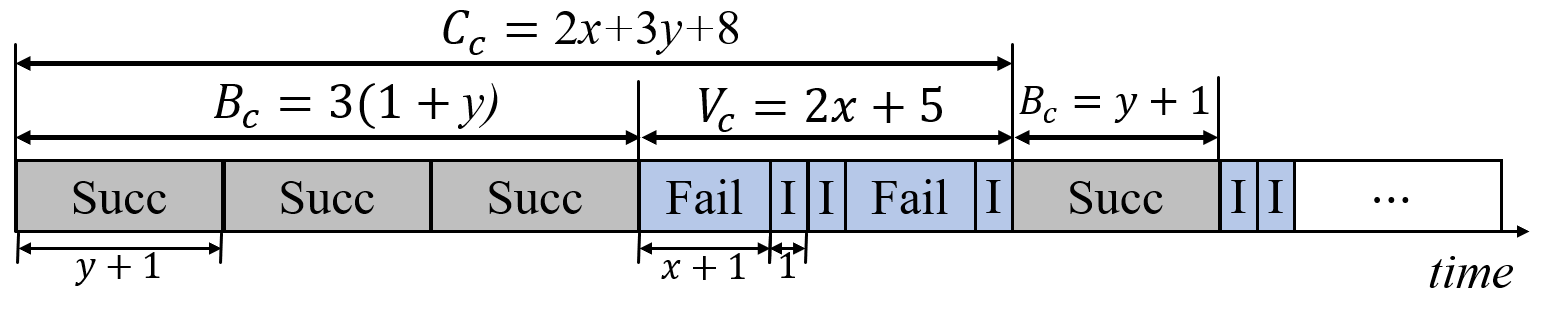
\includegraphics[width=0.9\textwidth]{figure/chap4/csmast_channel.png}
	\caption{CSMAST 方案中的信道状态演变示意图（$B$、$V_c$ 和 $C_c$ 分别表示信道的忙期、假期和周期时间）}
	\label{fig:csmast_channel}
\end{figure}

为了对 CSMAST 机制进行系统的定量分析，本小节引入离散时间休假排队理论作为建模基础。首先，我们将分析视角聚焦于信道的状态演变。从时间维度出发，CSMAST 网络中信道状态在连续占用与空闲/竞争阶段之间交替演化，呈现出明显的周期性特征。
图 \ref{fig:csmast_channel} 直观展示了 CSMAST 机制下的信道时序演化过程。基于上述信道时序演化过程的观察与抽象，对信道忙期与信道假期的概念作如下形式化定义：
\begin{itemize}
	\item \textbf{信道忙期 $B_c$}: 对应于图中连续出现的成功状态 S。在该阶段，某一节点成功占用信道，并通过连续传输机制持续发送数据包。从系统角度来看，该阶段对应于信道被有效利用以完成数据传输的过程。
	
	\item \textbf{信道假期 $V_c$}: 对应于图中碰撞状态 $F$ 与空闲状态 $I$ 的随机交替序列。
	该阶段刻画了上一忙期结束后，各节点为竞争下一次信道占用权所经历的接入过程。无论是由于多节点并发导致碰撞进入状态 $F$，还是由于无节点发送而处于状态 $I$，该阶段均对应于获取下一次成功接入所付出的时间开销与信令代价。
\end{itemize}
基于上述定义，将一次信道忙期与其后紧随的信道假期共同构成一个完整的信道周期，记为 $C_c$，即 $C_c = B_c + V_c$。
由于信道忙期由任一节点的成功接入所触发，且忙期一旦开始即由该节点独占信道并持续传输，因此从统计特性上看，信道层面的忙期与单节点视角下的忙期在概率分布上是等价的。为简化符号表示，后续分析中统一使用 $B$ 表示信道忙期。下文使用 $\overline{B} \triangleq \mathbb{E}[B]$ 和 $\overline{V}_c \triangleq \mathbb{E}[V_c]$ 分别表示信道忙期与信道假期的平均持续时长。具体的概率分布推导及性能指标计算将在下一节中进一步展开。

\section{基于休假排队理论的建模分析}
在进行具体推导之前，本节首先定义三个常用概率。根据第 ~\ref{subsec:channel_vacation_analysis}~节的分析，在饱和网络条件下，当节点数量 $n$ 较大且接入概率 $q$ 较小时，系统中的接入请求总数可近似建模为参数为 $\theta = nq$ 的泊松随机变量。在任意空闲时隙中，网络内发起接入请求的节点数量刻画了系统的瞬时竞争程度，并决定了下一时隙的信道状态转移。基于此，定义如下三个概率：
\begin{itemize}
	\item $p_0 = e^{-\theta}$：表示无节点发起接入请求的概率，即信道保持空闲状态。
	\item $p_1 = \theta e^{-\theta}$：表示恰有一个节点发起接入请求的概率，此时该节点成功占用信道并完成一次成功传输。
	\item $p_2 = 1 - p_0 - p_1$：表示至少有两个节点同时发起接入请求的概率，此时发生碰撞，对应信道进入失败状态。
\end{itemize}
下文将充分使用这三个概率，在所建立的休假排队模型中详细阐述忙期和假期分布规律。

\subsection{信道忙期 $B$ 分布的推导分析}
\label{subsec:B_analysis}
与第~\ref{chapter3:SAST}章所述的 SAST 机制类似，CSMAST 中的信道忙期分布取决于两个关键因素：一是当前占用节点是否持续发送，二是是否有其他节点发起接入请求并引发竞争。
在饱和网络假设下，当前已经成功接入的节点缓存始终非空，因此其在完成当前数据包传输后，将以概率 $1$ 持续发送后续数据包。
这意味着，信道忙期一旦开始，其终止不再依赖于发送节点的行为，而仅由其他节点发起接入请求所引发的碰撞事件所决定。
具体而言，一个信道忙期由若干个连续的成功传输状态 $S$ 构成，每个成功状态的持续时间为 $\tau_S$。在每个成功状态结束前的最后一个时隙（即侦听时隙）内，其余 $n-1$ 个节点对信道进行侦听，并据此判断得出信道将转入空闲态，从而可能发起新的接入请求。
根据前述的泊松近似，在该侦听时隙之后的下一时隙，网络中无其他节点发起接入请求的概率为$p_0 = e^{-\theta}$。此时系统可能出现以下两种情况：
\begin{itemize}
	\item 以概率 $p_0$，无其他节点发起接入请求，当前占用节点得以继续传输，信道状态由成功状态 $S$ 延续为新的成功状态，忙期持续。
	\item 以概率 $1 - p_0$，至少有一个其他节点发起接入请求，与当前节点的下一次传输发生冲突并引发碰撞，信道状态由成功状态 $S$ 转变为失败状态 $F$，从而终止当前忙期。
\end{itemize}
基于上述状态转移机制，忙期内连续成功传输的次数可建模为服从参数为 $1 - p_0$ 的几何分布，其中终止事件对应于碰撞的发生。考虑到每次成功传输的持续时间固定为 $\tau_S$，并且假设各成功状态之间的延续与终止事件相互独立，信道忙期的期望长度 $\overline{B}$可表示为：
\begin{equation}
	\overline{B} = \frac{\tau_S}{1 - p_0} = \frac{\tau_S}{1 - e^{-nq}}.
\end{equation}
进一步地，为评估系统服务过程的稳定性并支撑后续公平性分析，需要刻画信道忙期长度的波动特性。
基于前述几何分布建模结果，利用其方差表达式，信道忙期长度的方差 $\sigma_B^2$ 可表示为：
\begin{equation}
	\sigma^2_B = \tau_S^2 \cdot \frac{p_0}{(1 - p_0)^2} = \frac{ \tau_S^2 e^{-nq} }{(1 - e^{-nq})^2}.
\end{equation}
上述期望与方差从平均水平与波动程度两方面刻画了信道忙期特性。本质上，两者均由概率 $p_0$ 所主导。当 $p_0$ 较大时，节点在成功接入后更容易维持连续传输，平均占用信道的时间增加且波动性增强；反之，当 $p_0$ 较小时，忙期频繁终止，占用信道的时间更短且分布更集中。


\subsection{信道假期 $V_c$ 分布的推导与分析}
\label{subsec:Vc_analysis}
\begin{figure}[t]
	\centering
	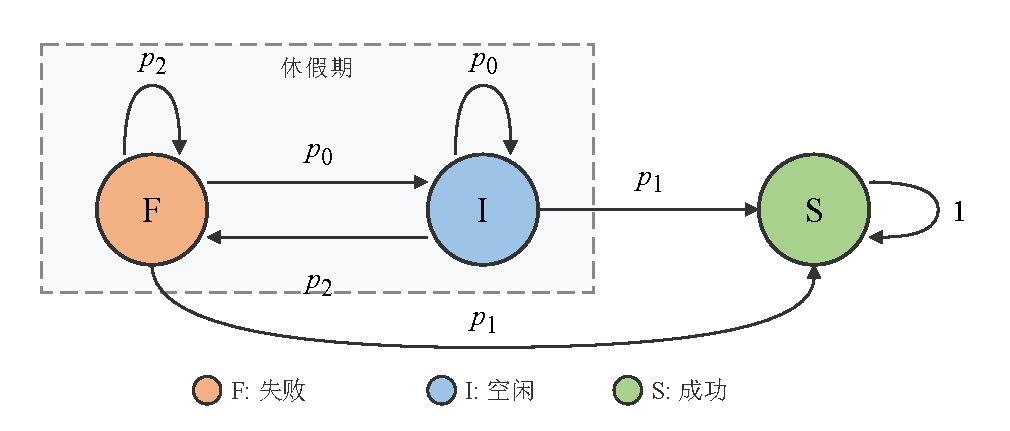
\includegraphics[width=0.95\textwidth]{figure/chap4/markov_model.pdf}
	\caption{描述信道假期 $V_c$ 内状态转移过程的吸收马尔可夫链模型（状态 F 和 I 为可转移态，状态 S 为吸收态）}
	\label{fig:csmast_markov_absorption}
\end{figure}

相较于仅包含成功传输的信道忙期，信道假期 $V_c$ 的演化更为复杂。
假期通常始于一次导致忙期终止的碰撞事件，此后信道在空闲与碰撞失败状态之间随机切换，直至某一时隙产生唯一成功传输，从而结束当前假期并开启新的信道忙期。
另一方面，空闲状态时长 $\tau_I$ 与碰撞状态时长 $\tau_F$ 并不相等，一般情况下 $\tau_F > \tau_I$。
因此，假期总时长不仅取决于状态转移情况，还与系统在不同状态下的驻留时间密切相关。
由于状态持续时间的非均匀性，基于独立同分布假设的几何分布模型难以准确刻画该过程的统计特性。
为推导信道假期分布特性，本文将在一个信道假期 $V_c$ 内，信道状态的演化过程建模为一个具有吸收态的马尔可夫链。该模型通过引入吸收态描述假期的终止事件，并刻画空闲状态与碰撞失败状态之间的随机转移关系，其状态转移结构如图 \ref{fig:csmast_markov_absorption} 所示。为形式化描述上述吸收马尔可夫链模型，本文首先构建其状态空间与转移概率矩阵，具体定义如下：

\begin{itemize}
	\item 模型包含三个状态。其中，碰撞状态 F 和空闲状态 I 构成瞬时状态集合，表示假期仍在持续；成功状态 S 是唯一的吸收态，一旦进入该状态，意味着某个节点竞争成功，假期结束并转入忙期。
	\item 在任意非忙期时隙，即状态 I 的时隙或状态 F 的最后一个侦听时隙，网络中发起接入请求总次数决定了下一时刻的状态跳转，有以下三个情况：
	\begin{enumerate}
		\item 无任何节点接入的概率为 $p_0 = e^{-\theta}$，此时信道保持静默，并进入空闲状态 I。
		\item 恰有一个节点发起接入的概率为 $p_1 = \theta e^{-\theta}$，此时信道进入成功状态 S，过程被吸收。
		\item 有多个节点同时接入的概率为 $p_2 = 1 - p_0 - p_1$，此时发生碰撞，信道进入碰撞状态 F。
	\end{enumerate}
\end{itemize}
基于上述转移逻辑，其状态转移概率矩阵 $\mathbf{P}$ 可表示为如下的标准分块形式：
\begin{equation}
	\mathbf{P} = 
	\begin{pmatrix}
		p_2 & p_0 & p_1 \\
		p_2 & p_0 & p_1 \\
		0 & 0 & 1
	\end{pmatrix}
	=
	\begin{pmatrix}
		\mathbf{T} & \mathbf{R} \\
		\mathbf{0} & \mathbf{I}
	\end{pmatrix},
\end{equation}
其中，$\mathbf{T} = \begin{pmatrix} p_2 & p_0 \\ p_2 & p_0 \end{pmatrix}$ 描述了瞬态之间的转移概率，$\mathbf{R} = \begin{pmatrix} p_1 \\ p_1 \end{pmatrix}$ 描述了进入吸收态的概率。
根据马尔可夫吸收理论\cite{2008_Markov_absorb}，相关性能指标的计算依赖于基本矩阵 $\mathbf{N} = (\mathbf{I} - \mathbf{T})^{-1}$。其中，矩阵 $\mathbf{N}$ 中的元素 $N_{ij}$ 表示过程从瞬时状态 $i$ 开始，在被吸收之前访问到瞬时状态 $j$ 的期望次数。本节中，矩阵 $\mathbf{N}$ 的行、列索引按顺序分别对应状态 F 和状态 I。
首先计算矩阵 $(\mathbf{I} - \mathbf{T})$：
\begin{equation}
	\mathbf{I} - \mathbf{T} = 
	\begin{pmatrix} 1 & 0 \\ 0 & 1 \end{pmatrix} - \begin{pmatrix} p_2 & p_0 \\ p_2 & p_0 \end{pmatrix} 
	= \begin{pmatrix} 1-p_2 & -p_0 \\ -p_2 & 1-p_0 \end{pmatrix}.
\end{equation}
其行列式为 $\det(\mathbf{I} - \mathbf{T}) = (1-p_2)(1-p_0) - p_0 p_2 $。
结合概率归一化关系 $p_0 + p_1 + p_2 = 1$，求解基本矩阵 $\mathbf{N}$为
\begin{equation}
	\mathbf{N} = \frac{1}{p_1} \begin{pmatrix} 1-p_0 & p_0 \\ p_2 & 1-p_2 \end{pmatrix}.
\end{equation}

在饱和网络条件下，信道假期均由碰撞状态触发，因而仅需关注从碰撞状态 $F$ 出发的期望访问次数。根据基本矩阵定义，$N_{FF} = (1-p_0)/p_1$ 表示在吸收之前访问碰撞状态 $F$ 的期望次数，对应假期内经历的平均碰撞次数，$N_{FI} = p_0/p_1$ 为空闲状态 $I$ 的期望次数，对应假期内经历的平均空闲次数。
令列向量 $\boldsymbol{\mu} = [\tau_F, \tau_I]^T$ 表示各瞬时状态的单次驻留时长，则从各瞬态出发至吸收态的期望总时间向量 $\mathbf{F}$ 可表示为 $\mathbf{F} = \mathbf{N} \boldsymbol{\mu}$。
取向量 $\mathbf{F}$ 的第一个分量，对应初始状态 F。代入 $p_0 = e^{-\theta}$、$p_1 = \theta e^{-\theta}$ 以及 $\theta = nq$，即可得到信道假期的期望长度为：
\begin{equation}
	\overline{V}_c = [\mathbf{F}]_1 = [\mathbf{N} \boldsymbol{\mu}]_1 = \frac{1-p_0}{p_1}\tau_F + \frac{p_0}{p_1}\tau_I = \frac{(1 - e^{-nq})\tau_F + e^{-nq}\tau_I}{nq e^{-nq}}.
\end{equation}

为了分析公平性，还需计算假期长度 $V_c$ 的二阶统计量。根据吸收马尔可夫链理论，从各瞬态出发至吸收态的总时间二阶矩向量 $\mathbf{G}$ 满足
\begin{equation}
	\mathbf{G} = \mathbf{N} ( \mathbf{m}_2 + 2 \cdot \text{diag}(\boldsymbol{\mu}) \cdot \mathbf{T} \mathbf{F} ),
\end{equation}
其中 $\mathbf{m}_2 = [\tau_F^2, \tau_I^2]^T$ 为各瞬态单次驻留时间的二阶矩向量，$\text{diag}(\boldsymbol{\mu})$ 为以 $\boldsymbol{\mu}$ 为对角元素的对角矩阵。
提取向量 $\mathbf{G}$ 的第一个分量，可以得到从状态 F 出发至吸收态的假期长度的二阶原点矩 $\mathbb{E}[V_c^2] = \mathbf{G}_1$。因此，信道假期的方差 $\sigma^2_{V_c}$ 由公式 $\sigma^2_{V_c} = \mathbf{G}_1 - (\overline{V}_c)^2$ 给出：
\begin{equation}
	\sigma^2_{V_c} =
	\frac{\left[(1 - p_0)\tau_F + p_0\tau_I\right]^2}{p_1^2} - \frac{(1 - p_0)\tau_F^2 + p_0\tau_I^2}{p_1}.
\end{equation}


\subsection{信道周期 $C_c$ 与节点周期 $C$ 的推导与分析}
\label{subsec:cycle_analysis}

基于前文对信道忙期 $B$ 和信道假期 $V_c$ 的独立分析，下面推导完整信道周期 $C_c$ 以及节点周期 $C$ 的统计特性。这一推导能够表征系统的时间演化规律，周期长度的方差将直接决定系统的短期公平性性能。

首先分析信道周期 $C_c$ 的均值与方差。根据休假排队模型定义，一个完整的信道周期 $C_c$ 由一个忙期 $B$ 和随后的一个假期 $V_c$ 构成，满足关系式 $C_c = B + V_c$。
在 CSMAST 机制下，信道忙期长度取决于当前占用节点的连续发送意愿以及碰撞发生概率，信道假期长度取决于碰撞和空闲状态跳转。需要注意的是，假期开始意味着上一次忙期的状态记忆被完全重置，碰撞会使得所有节点重新参与信道竞争，因此在系统平稳情况下，随机变量 $B$ 与 $V_c$ 可被视为相互独立。

依据概率论中独立随机变量和的基本性质，信道周期的均值$\overline{C}_c$和方差$\sigma^2_{C_c}$ 可由其组成部分的统计量线性叠加得到，即
\begin{equation}
	\overline{C}_c = \overline{B} + \overline{V}_c,
\end{equation}
\begin{equation}
	\sigma^2_{C_c} = \sigma^2_B + \sigma^2_{V_c}.
\end{equation}
式中$\overline{B}$和$\sigma^2_B$在\ref{subsec:B_analysis}节已经得出，$\overline{V}_c$和$\sigma^2_{V_c}$在\ref{subsec:Vc_analysis}节中推导。该结果完整刻画了信道资源在占用状态与争夺状态之间切换的时间特征。

然后分析节点周期$C$及其方差$\sigma^2_C$的映射关系。
为刻画节点间的公平性特征，本文将分析视角由信道转向单节点。与第~\ref{chapter3:SAST}章类似，定义节点周期 $C$ 为某一特定节点两次连续接入信道并开启忙期之间的时间间隔。
在包含 $n$ 个同质节点的饱和网络中，各节点具有一致的统计特性，且传输概率 $q$ 相同。每一次成功接入对应一个完整的信道周期 $C_c$，并以相同概率 $1/n$ 归属于任意一个节点。对于某一指定节点而言，其成功接入信道的过程可等效视为在信道周期序列上进行一次以 $1/n$ 为采样概率的随机稀疏采样过程。
换言之，对于任一给定节点，其平均需要经历约 $n$ 个信道周期后才能成功接入信道。因此，节点周期的均值 $\overline{C}$ 与信道周期均值 $\overline{C}_c$ 之间满足如下线性比例关系：
\begin{equation}
	\overline{C} = n \overline{C}_c.
\end{equation}

结合更新过程理论中关于点过程稀疏化的相关结论，当网络节点规模 $n$ 较大且信道周期之间的相关性较弱时，节点周期的方差 $\sigma^2_C$ 与信道周期方差 $\sigma^2_{C_c}$ 之间存在近似关系：
\begin{equation}
	\label{eq:node_cycle_variance}
	\sigma^2_C \approx n^2 \sigma^2_{C_c} - (1 - n)n\overline{C}_c \approx n^2 \sigma^2_{C_c}.
\end{equation}
上式中的近似 $\sigma^2_C \approx n^2 \sigma^2_{C_c}$ 是基于 $n$ 较大时第一项占主导地位而得到的。

该结论表明，节点周期的波动性会随着信道周期的波动而发生变化，并被网络规模 $n$ 的平方放大。结合前文分析结论，当传输概率 $q$ 取值较小时，信道忙期的方差 $\sigma^2_B$ 数值较大，存在节点长时占用信道的可能，进而导致信道周期方差 $\sigma^2_{C_c}$ 增大，再通过上述方差映射关系放大节点周期的波动幅度。这种较大的服务间隔波动，从数学上揭示了 CSMAST 机制在提升系统吞吐量的同时可能牺牲节点间公平性的内在原因，也为下一节推导 Jain 公平性指数奠定了理论基础。


\section{吞吐量与公平性指标的推导与分析}
\label{sec:csmast_performance}

基于前文构建的休假排队模型及信道与节点周期的统计特性，本节将推导 CSMAST 网络在饱和状态下的两个核心性能指标，即网络吞吐量与 Jain 公平性指数。这不仅能够定量评估该机制的传输效率，还能揭示连续传输策略在系统效率与用户公平之间的内在权衡关系。

\subsection{网络吞吐量指标的推导与分析}

网络吞吐量 $\lambda^{net}_{out}$ 定义为单位时间内信道成功传输的有效数据数量，以包/时隙为单位。
在计算该指标时，必须考虑成功状态 S 的特殊性。虽然成功状态持续 $\tau_S$ 个时隙，但其中仅有 $y$ 个时隙用于实际数据包传输，剩余的 1 个时隙被用于必要的信道侦听。因此，信道忙期 $\overline{B}$ 并不能完全代表有效吞吐时间，需引入修正因子 $\frac{\tau_S - \tau_I}{\tau_S} = \frac{y}{y+1}$。
结合前文推导的 $\overline{B}$ 和 $\overline{V}_c$ 表达式，饱和状态下的网络吞吐量可表示为：
\begin{equation}
	\lambda^{net}_{out} = \frac{\tau_S - \tau_I}{\tau_S} \cdot \frac{\overline{B}}{\overline{B} + \overline{V}_c}.
\end{equation}
将 $p_0 = e^{-nq}$ 及 $\overline{B}, \overline{V}_c$ 关于网络参数的表达式代入，得到 CSMAST 网络吞吐量的闭式表达式为
\begin{equation}
	\label{eq:throughput_csmast}
	\lambda^{net}_{out} = \frac{nq(\tau_S - \tau_I)}{nq\tau_S + e^{nq}(1 - e^{-nq})^2 \tau_F + (1 - e^{-nq})\tau_I}.
\end{equation}
基于上述结果，进一步给出 CSMAST 吞吐量极限的如下定理：

\begin{theorem}[CSMAST 最大网络吞吐量]
	\label{thm:csmast_max_throughput}
	在饱和状态下，CSMAST 的网络吞吐量是关于参数 $nq$ 的单调递减函数。其理论最大吞吐量在接入概率 $q \to 0$ 时取得：
	\begin{equation}
		\lambda_{max}^{net} = \lim_{nq \to 0} \lambda^{net}_{out} = \frac{\tau_S - \tau_I}{\tau_S + \tau_I}.
	\end{equation}
\end{theorem}

\begin{proof}
	对于单调性，令 $x = nq$。饱和网络吞吐量可表示为 $g(x) = \frac{C x}{x \tau_S + F(x)}$，其中 $C = \tau_S - \tau_I > 0$，分母中的信道假期相关项为 $F(x) = \tau_F e^x (1 - e^{-x})^2 + \tau_I (1 - e^{-x})$。
	对 $g(x)$ 求导，其导数的符号完全取决于分子部分的判别式 $T(x) \triangleq F(x) - x F'(x)$。将 $F(x)$ 及其导数代入，并利用基本不等式 $1 - e^{-x} \le x$ 和 $e^{-x} \le 1$（对于 $x > 0$），可以证明在通常的系统参数设定下（即 $\tau_F \ge \tau_I$），判别式满足 $T(x) \le 0$。
	由于 $g'(x)$ 与 $T(x)$ 同号，因此 $g'(x) \le 0$ 在定义域内恒成立。这证明了 CSMAST 的网络吞吐量是关于 $nq$ 的单调递减函数。
	
	对于最值，利用洛必达法则对式 (\ref{eq:throughput_csmast}) 在 $nq \to 0$ 处求极限。注意到分母中 $e^{nq}(1-e^{-nq})^2 \approx (nq)^2$ 为高阶小量，主要项为 $(1-e^{-nq})\tau_I \approx nq \tau_I$。分子近似为 $nq(\tau_S - \tau_I)$。分子分母约去 $nq$ 后，第一项 $nq\tau_S$ 趋于 0，剩余部分即为极限值 $\frac{\tau_S - \tau_I}{\tau_S + \tau_I}$。
\end{proof}

定理 \ref{thm:csmast_max_throughput} 给出了 CSMAST 的最大理论吞吐量。以典型参数配置 $\tau_S=5, \tau_F=3, \tau_I=1$ 为例，CSMAST 的理论极限吞吐量可达 $4/6 \approx 0.667$，而相同参数下的经典 CSMA 仅能达到约 0.518，对应约 28.8\% 的吞吐量提升。这表明 CSMAST 通过连续传输机制，将空闲侦听 $\tau_I$ 和碰撞退避 $\tau_F$ 的时间成本分摊到连续多个数据包传输过程中，从而降低单位数据包的平均接入成本。

值得指出的是，本文所构建的基于吸收马尔可夫链的休假排队模型具有良好的扩展性与统一性。CSMAST 机制的性能增益本质上来源于连续传输机制增加了平均信道忙期 $\overline{B}$。作为该模型的一种特例，若在分析中约束节点在完成单个数据包传输后必须立即释放信道，即将忙期退化为确定性常数 $\overline{B} = \tau_S$，则所建立的模型可自然退化为对经典 CSMA 协议的性能刻画。在该情形下，系统不再具备连续占用信道的能力，其信道接入行为与传统 CSMA 机制一致。因此，经典 CSMA 协议可视为本文模型在特定参数约束下的一个退化情形。
关于经典 CSMA 在本章相同模型框架下的详细推导及最大吞吐量计算，详见附录\ref{app:classic_csma}。综上，该理论联系不仅验证了所提模型在不同接入机制下的一致性与通用性，同时也为后续性能对比分析提供了统一的数学基准。

\subsection{公平性指标的推导与分析}

尽管连续传输机制提升了系统吞吐量，但其一旦接入便持续占用信道的特性不可避免地对节点间的公平性构成挑战。为了量化这一影响，本节采用短期 Jain 公平性指数 $J_T$ 作为评估指标，并基于前文推导其闭式解。

设 $\lambda_{out, i}^T$ 为节点 $i$ 在给定观测时间窗 $T$ 内的短期归一化吞吐量。Jain 公平性指数定义为
\begin{equation}
	J_T = \frac{\left(\sum_{i=1}^n \lambda_{out, i}^T\right)^2}{n \sum_{i=1}^n \left(\lambda_{out, i}^T\right)^2}.
\end{equation}
由于网络中所有节点是同质的，$\lambda_{out, i}^T$ 可视为一组独立同分布的随机变量。根据大数定律，当节点数量 $n$ 足够大时，上述定义表达式可以写成
\begin{equation}
	\label{eq:jain_moment_form}
	J_T \approx \frac{\mathbb{E}[\lambda_{out, i}^T]^2}{\mathbb{E}[(\lambda_{out, i}^T)^2]} = \frac{1}{1 + \frac{\text{Var}(\lambda_{out, i}^T)}{\mathbb{E}[\lambda_{out, i}^T]^2}}.
\end{equation}
因此，求解 $J_T$ 的关键在于推导短期内节点吞吐量的均值 $\mathbb{E}[\lambda_{out, i}^T]$ 和方差 $\text{Var}(\lambda_{out, i}^T)$。

在 CSMAST 饱和网络中，节点 $i$ 的成功接入过程构成一个更新过程。令 $N_i(T)$ 表示节点 $i$ 在时间 $T$ 内成功完成的节点周期数，即节点经历的忙期次数。节点的短期吞吐量可表示为单位时间内传输的数据包总量：
\begin{equation}
	\lambda_{out, i}^T \approx \frac{N_i(T) \cdot \overline{B}}{T}.
\end{equation}
当观测时间 $T$ 充分长，即 $T \gg \overline{C}$ 时，根据更新理论的渐近性质\cite{1996_Gausian}，计数过程 $N_i(T)$ 近似服从正态分布，其均值和方差分别为：
\begin{equation}
	\mathbb{E}[N_i(T)] \approx \frac{T}{\overline{C}}, \quad \text{Var}(N_i(T)) \approx \frac{\sigma^2_C}{\overline{C}^3} T.
\end{equation}
基于此，短期吞吐量的统计特征总结为：
\begin{equation}
	\mathbb{E}[\lambda_{out, i}^T] = \frac{\overline{B}}{\overline{C}}, \quad \text{Var}(\lambda_{out, i}^T) = \left( \frac{\overline{B}}{T} \right)^2 \times \text{Var}(N_i(T)) = \frac{\overline{B}^2 \sigma^2_C}{\overline{C}^3 T}.
\end{equation}
将上述均值和方差代入式 (\ref{eq:jain_moment_form})，化简并展开可得到 Jain 公平性指数的闭式表达式：
\begin{equation}
	\label{eq:jain_explicit}
	J_T \approx \frac{1}{1 + \frac{n}{T} \cdot \frac{n^2 q^2 \tau_S^2 e^{nq} + (e^{nq}-1)^2 \tau_F^2 + 2(e^{nq}-1)\tau_F \tau_I + \tau_I^2}{nq \tau_S e^{nq} + (e^{nq}-1)^2 \tau_F + (e^{nq}-1)\tau_I}}.
\end{equation}
\section{仿真验证与结果分析}
\label{sec:simulation_results}


本节通过蒙特卡洛仿真从三个层面验证前文结论：理论一致性、与经典 CSMA 的对比增益、以及机制层面的性能权衡。仿真平台基于 MATLAB 构建，严格遵循第 4.1 节定义的异构时隙结构与碰撞信道模型。在所有仿真中，网络处于饱和状态，节点仅在侦听到信道可用时才以概率 $q$ 在下一时隙发起接入。
在仿真中，网络吞吐量按
$\lambda^{net}_{out}=\frac{N_{succ}(\tau_S-\tau_I)}{T}$
计算，其中 $N_{succ}$ 表示观测窗口内总体成功接入次数，$T$ 为总仿真时长。
短期公平性由各节点短期吞吐量按 Jain 指数标准定义计算，即
$J_T=\frac{\left(\sum_{i=1}^{n}\lambda_{out,i}^{T}\right)^2}{n\sum_{i=1}^{n}(\lambda_{out,i}^{T})^2}$。
其中节点 $i$ 的短期吞吐量按
$\lambda_{out,i}^{T}=\frac{N_{succ,i}(\tau_S-\tau_I)}{T}$
计算，$N_{succ,i}$ 表示节点 $i$ 在观测窗口内的成功数据包数量。
% 除非另有说明，本节采用基准参数 $n=100$、$T=10^6$、$x=2$、$y=4$，即 $\tau_I=1,\tau_F=3,\tau_S=5$，并在图注中明确对应的观测窗口。

\subsection{网络吞吐量 $\lambda^{net}_{out}$ 的仿真验证与分析}

\begin{figure}[t]
	\centering
	\begin{subfigure}{0.49\textwidth}
		\centering
		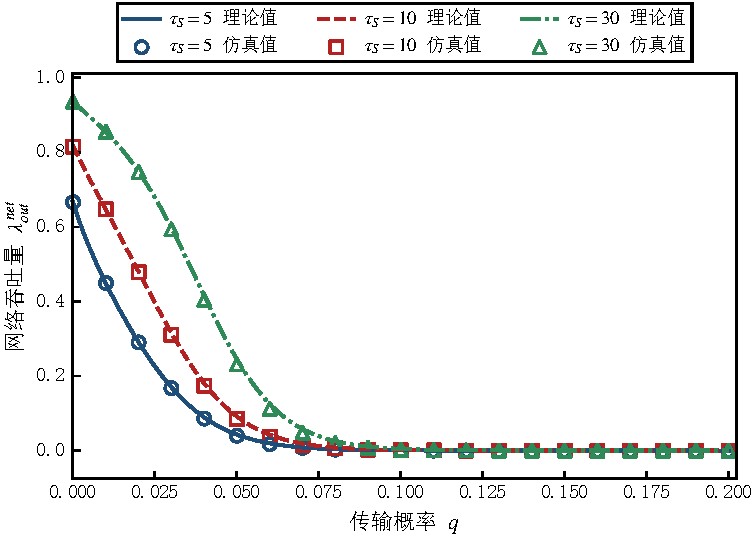
\includegraphics[width=\linewidth]{figure/chap4/thu_vs_q_CSMAST_multi_taus.pdf}
		\caption{不同 $\tau_S$ 下 $\lambda^{net}_{out}$ 随接入概率 $q$ 的变化情况}
		\label{fig:csmast_throughput_vs_q_taus}
	\end{subfigure}
	\hfill
	\begin{subfigure}{0.49\textwidth}
		\centering
		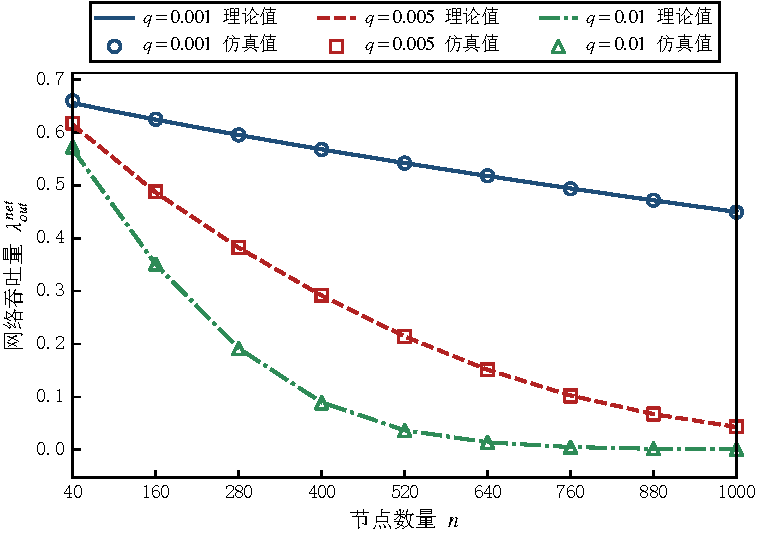
\includegraphics[width=\linewidth]{figure/chap4/thu_vs_n_CSMAST_multi_q.pdf}
		\caption{网络吞吐量 $\lambda^{net}_{out}$ 随节点数量 $n$ 的变化情况}
		\label{fig:csmast_throughput_vs_n}
	\end{subfigure}
	\caption{CSMAST 机制下吞吐量随系统参数变化情况}
	\label{fig:csmast_throughput_group}
\end{figure}

图 \ref{fig:csmast_throughput_vs_q_taus} 给出了不同成功传输时长 $\tau_S$ 条件下，网络吞吐量 $\lambda^{net}_{out}$ 随接入概率 $q$ 变化的曲线趋势。实验参数设置为节点数 $n=100$、碰撞时长 $\tau_F=3$、空闲时长 $\tau_I=1$、观测时间窗口 $T=10^6$，并取 $\tau_S\in\{5,10,30\}$。结果显示，在相同接入概率 $q$ 下，$\tau_S$ 越大，吞吐量曲线整体越高。该现象说明成功传输阶段越长，单位成功发送的数据包所经历的时间开销越低，从而提升了网络吞吐量。随着 $q$ 增大，三组曲线均持续下降，原因在于并发接入概率上升导致碰撞频率增加，有效传输时间占比下降。在较大 $q$ 区域，曲线间距逐步收敛，表明系统性能主要受高冲突过程主导，$\tau_S$ 带来的增益受到削弱。理论曲线与仿真结果在全区间内保持一致，验证了理论对该参数变化规律的准确性。

\begin{figure}[t]
	\centering
	\begin{subfigure}{0.49\textwidth}
		\centering
		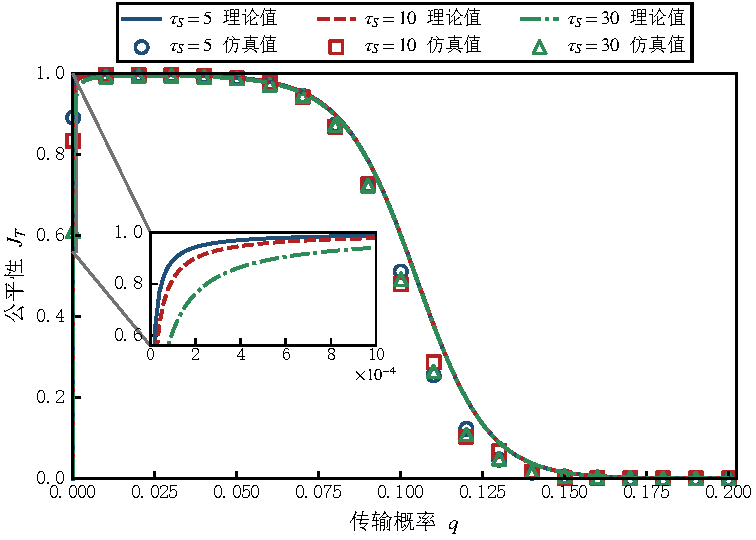
\includegraphics[width=\linewidth]{figure/chap4/jt_vs_q_CSMAST_multi_taus.pdf}
		\caption{不同 $\tau_S$ 下公平性 $J_T$ 随接入概率 $q$ 的变化情况}
		\label{fig:csmast_jain_vs_q_taus}
	\end{subfigure}
	\hfill
	\begin{subfigure}{0.49\textwidth}
		\centering
		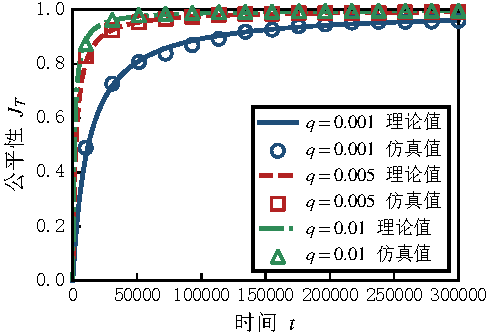
\includegraphics[width=\linewidth]{figure/chap4/jt_vs_t_CSMAST_multi_q.pdf}
		\caption{不同 $q$ 下短期公平性 $J_T$ 随观测时间窗口 $T$ 的变化情况}
		\label{fig:csmast_jain_vs_t_multi_q}
	\end{subfigure}
	\caption{CSMAST 机制下公平性关于系统参数的变化情况}
	\label{fig:csmast_fairness_group}
\end{figure}

为考察网络规模影响，图~\ref{fig:csmast_throughput_vs_n} 给出了不同接入概率 $q$ 条件下网络吞吐量 $\lambda^{net}_{out}$ 随节点数量 $n$ 变化的趋势。实验参数设置为成功传输时长 $\tau_S=5$、碰撞时长 $\tau_F=3$、空闲时长 $\tau_I=1$、观测时长 $T=10^6$。结果显示，在任一固定 $q$ 下，$n$ 增大将提高总体竞争强度，并增加碰撞与侦听带来的时间开销，使吞吐量整体下降；在任一固定 $n$ 下，较小 $q$ 往往对应更高吞吐量，但也会伴随更明显的公平性代价。
% 理论与仿真曲线的总体一致性说明该模型在不同负载区间均具有较好解释力。

\subsection{公平性 $J_T$ 的仿真验证与分析}


图 ~\ref{fig:csmast_jain_vs_q_taus} 进一步给出了不同 $\tau_S$ 下短期公平性 $J_T$ 随接入概率 $q$ 的变化趋势。实验参数设置为节点数 $n=100$、碰撞时长 $\tau_F=3$、空闲时长 $\tau_I=1$，观测时长 $T=10^6$，并取 $\tau_S\in\{5,10,30\}$。该图表明，在低接入概率区间，$\tau_S$ 越大，$J_T$ 越低，说明连续忙期越长，节点间短时服务差异越明显。随着 $q$ 增大，碰撞对信道连续占用的中断效应增强，增加了信道占用权在节点之间的轮转，$J_T$ 因而逐步上升。进入高接入概率区间后，$J_T$ 逐渐下降并且不同 $\tau_S$ 下的公平性曲线逐渐收敛，说明公平性主要由竞争过程主导，而忙期长度差异的影响相对减弱。
% 理论曲线与仿真点在全区间保持一致，进一步验证了第 4.3 节公平性模型的有效性。

\begin{figure}[t]
	\centering
	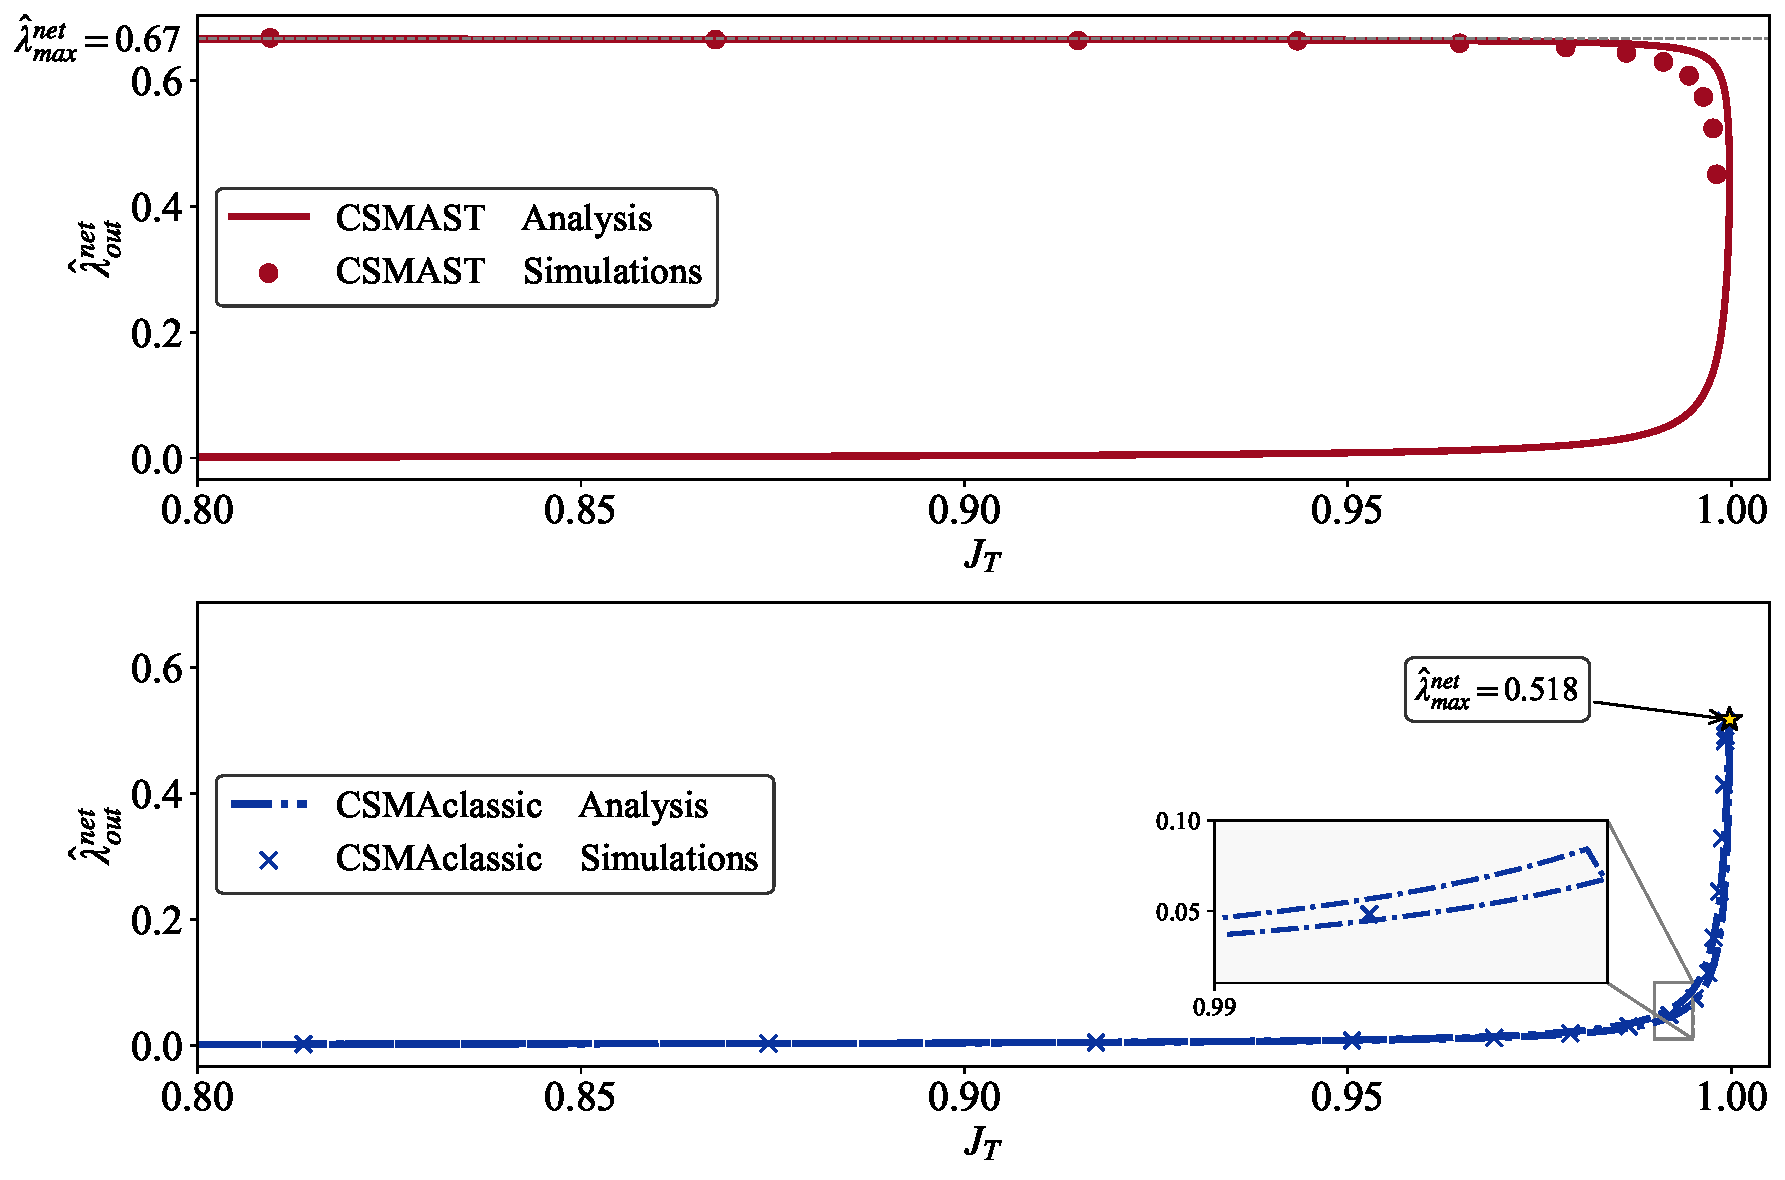
\includegraphics[width=0.7\textwidth]{figure/chap4/throughput_fairness_tradeoff.pdf}
	\caption{CSMAST 与经典 CSMA 机制的吞吐量-公平性轨迹对比（$n=100,\tau_S=5,\tau_F=3,\tau_I=1,T=10^6$）}
	\label{fig:comparison_classic}
\end{figure}

图~\ref{fig:csmast_jain_vs_t_multi_q} 进一步展示了不同接入概率 $q$ 下短期公平性 $J_T$ 随观测时间窗口 $T$ 的变化。实验参数设置为节点数 $n=100$、成功传输时长 $\tau_S=5$、碰撞时长 $\tau_F=3$、空闲时长 $\tau_I=1$。不同 $q$ 条件下理论曲线与仿真结果保持一致。结果表明，随着观测窗口增大，$J_T$ 整体上升并逐步趋于稳定，这与式 \ref{eq:jain_explicit} 中公平性随 $T$ 增大而改善的理论相符。可见，较短观测窗口内统计量更易受到连续忙期波动影响，节点间服务差异更明显；当观测窗口扩展后，碰撞重分配与多轮接入过程得到充分平均，短时不公平被逐步平滑。

\subsection{CSMAST 与 CSMA 机制的性能对比与分析}

图 \ref{fig:comparison_classic} 进一步展示了 CSMAST 与经典 CSMA 方案在吞吐量与公平性二维平面上的性能轨迹对比。对比实验采用统一参数设置：节点数 $n=100$、成功传输时长 $\tau_S=5$、碰撞时长 $\tau_F=3$、空闲时长 $\tau_I=1$，观测时长 $T=10^6$。经典 CSMA 的性能曲线基于附录\ref{app:classic_csma} 中推导的理论公式所绘制，保证两者是在完全相同的时隙结构参数 $x, y$ 以及统一分析框架下进行比较。通过遍历传输概率 $q$，可以得到两种方案在不同工作点下的性能包络。对比结果表明，在同等公平性水平下，CSMAST 的吞吐量高于经典 CSMA。具体而言，经典 CSMA 的最大理论吞吐量约为 0.518，而 CSMAST 可提升至 0.667，对应约 28.8\% 的吞吐量提升。

进一步分析可知，在低吞吐量区间（$\lambda^{net}_{out}<0.518$，对应较大 $q$）两种机制轨迹近乎重合。其原因是强竞争使信道在空闲与碰撞状态间高频切换，从而令两者的假期基本一致；此时性能差异主要由忙期 $\overline{B}$ 决定。随着 $q$ 减小，CSMAST 通过连续传输拉长 $\overline{B}$ 并提升吞吐量；随着 $q$ 增大，碰撞使忙期退化至近单包时长，机制行为趋近经典 CSMA。连续传输会在短时间尺度放大服务不对称现象并影响瞬时公平性，但其对假期的分布特性的影响有限，因此在长期统计意义下，两种机制的 Jain 指数保持接近。综上，CSMAST 可通过较小 $q$ 在可控公平代价下获得吞吐量增益。

\section{本章小结}

本章针对载波侦听接入网络的性能瓶颈，提出了基于连续传输的 CSMAST 机制。考虑到 CSMA 协议的状态时长异构性，本章引入吸收马尔可夫链理论，构建休假排队分析框架，成功推导了饱和状态下网络吞吐量与 Jain 公平性指数的闭式解。
理论与仿真分析表明，在一组相同配置条件下，CSMAST 相比传统 CSMA 实现了约 28.8\% 的吞吐量提升，同时还能保持较好的公平性。

